\chapter{Basic Types and Control Flow}

Computers work with data. At the lowest level, this data is just `on' and
`off' in a transistor. Software craftsmen don't work at this level. Instead,
our programming languages give us the tools to work with this data in a much
more intuitive fashion. In broad strokes, this is achieved with two concepts:
data types and control flow. Data types describe the data our program is
working with, whether it be a number, a bank account, or an image. Control
flow describes the operations that occur on the data over time, like adding
numbers, checking the balance of a bank account, or cropping an image.

You can think of data types as the space of a program. At any one point in
time, we will have certain sets of data we are working with. We can stop the
program, look at the data, and carry on. While we think of three dimensions in
space,  up/down, left/right, and front/back, there are many more dimensions we
could talk about for different things. A table has a color, along with its
position. Our programs represent these properties in different ways, but we as
programmers abstract them, and the term we use to talk about these properties
is data types.

Control flow would then be the time aspect of a program. As the program runs,
it does different things to the data. At some point, it might need to make a
decision, and do one thing or another depending on what properties the data
has. At another point, the program might need to do the same thing on a bunch
of similar pieces of data. Control flow represents the logical actions our
programs follow.

\section{Syntax}

Before we dive into discussing our first program, there is one more topic to
cover. Syntax describes the words and symbols that make a valid program. In
English, nouns, verbs and adjectives must come in a certain fashion for a
sentence to make sense. In a computer program, there are similar rules for how
a program can be written, and still make sense to the computer to run. We will
cover the details of syntax for each programing language in the workbook, but
there are some key terms to know regardless of the language.

\subsection{Keywords}

In any programming language, there are a few reserved {\it keywords} --- words
which have a specific meaning to the program. Most programming languages only
use no more than a couple dozen keywords. These will be covered in the
workbooks as needed.

\subsection{Variables}

In a program file, variables are words used to refer to some piece of data.
Variables let programmers use concrete concepts to refer to the more abstract
realm of the mathematical values in the computer. Variables can generally be
any word that isn't a keyword in a programming language.

\subsection{Operators}

Operators are the built-in things that can happen to data. Common operators
are things from elementary arithmetic --- add {\tt +}, subtract {\tt -},
multiply {\tt *}, and divide {\tt /}. Other operators let the program compare
two pieces of data --- equals ({\tt ==}), less-than ({\tt <}), greater-than-
or- equal-to ({\tt >=}). Notice there are some funny things for the comparison
operators. First, equals is two characters, {\tt ==}, not the single {\tt =}
used in elementary school. This is because a single {\tt =} sign is an
operator used to assign values to a variable. Multiplication is a star, {\tt
*}. While {\tt x} was used in elementary school, we use {\tt *} for our
programs because {\tt x} could be a variable, and we need to be unambiguous in
what the program means. There is no $\le$ on a common keyboard, so programs
use the two character combinations of {\tt <=} and {\tt >=} to do comparisons.
There are other operators that will be covered as they are needed.

\section{Basic Types}

Data Types fall into two distinct categories. `Primitive' data types are those
that are specified in the programming language itself. `Complex' data types
are defined by the programmer, and are made up entirely of primitive data
types and other complex data types already defined. In this section, we will
go over the basic data types in your language. In general, these basic types
are applicable in any programming language in major use today, with small
discrepencies between them.

\subsection{Numbers}

Since computers only do arithmetic, everything is at some level a number in
the computer. In mathematics, numbers can be as big as they need to be. If we
were counting pebbles of sand on a beach, there is a number to represent that
(though I will not be the one doing the counting). Computers are somewhat more
finite. The representation of a basic number in a computer is confined to a
range of a few possible values. On today's computers, that range is either
$2^32$ or $2^64$ possible values. The 32 and 64 refer to the number of `bits'
your computer handles. When the IT guy asks whether your computer is 32 or 64
bit, this is what we're talking about.

\subsubsection{Integers}

Integers in computer programming are Whole Numbers from elementary school ---
1, 5, -15, 47. They can be positive or negative. In some languages, they are
limited in size based on your computer's processor. On a 32 bit computer, the
range of integers is from $-2^{31}$ (-2 147 483 648) to $2^{31}-1$ (2 147 483
647) (the one positive number is lost for 0). On a 64 bit computer, the range
of values is $-2^{63}$ to $2^{63}-1$. It is left to the reader to determine
those numbers in base 10. Integers are useful in many cases because they are
very easy to work with, but have a major drawback of being unable to work with
fractional parts. That is the use of Floating-point numbers.

\subsubsection{Floats}

In your computer, there is only so much room to store numbers. As mentioned in
the previous section on integers, there are only $2^32$ possible numbers you
can represent on a 32-bit computer. Those integers are only whole numbers, and
can't represent a number like $\frac{1}{2}$ or $\pi = 3.1415926...$. Instead,
we use a special type of number called a {\em Floating Point} number. A
floating point number can still only represent $2^32$ different values, but it
is interpreted in such a way that it can represent fractional numbers. At this
point, we must take a detour into the world of mathematics in order to
understand how floating point numbers work, and in the process save ourselves
from making some very costly mistakes.

{\bf Floating Point Arithmetic}\
This section explains some complicated math.\

Our everyday number system is a base-10 number system. When you write your
numbers, you write 1, 2, 3, 4, 5, 6, 7, 8, 9, 10, 11, 12 $...$. Notice how
starting at 10 we use two characters to represent the number- 1 and 0. ``Well,
duh" you might say. In fact, there is a very specific reason we need two
numbers at this point. What 10 means is $(1 * 10^1) + (0 * 10^0)$. This is the
base-10 system- each character in the numer means $a * 10 ^ p$ where $a$ is
the number, and $p$ is its position (starting from 0). So, the number 347 is
$(3 * 10 ^ 2) + (4 * 10 ^ 1) + (7 * 10^0)$. In a computer, we use binary, or a
base-2 number  system. Instead of writing numbers as $a * 10^p$, we write them
as $a * 2 ^ p$. So, to get 12, we need to write 1100, or $(1 * 2 ^ 3) + (1 *
2^2) + (0*2^1) + (0 * 2 ^ 0) = (1 * 8) + (1 * 4) + (0 * 2) + (0 * 1) = 8 + 4 +
0 + 0 = 12_10$.

We can talk about decimal numbers like 1.56 in the same way--- $(1 * 10 ^ 0) +
(5 * 10 ^ -1) * (6 * 10 ^ -2) = 1 + \frac{5}{10} + \frac{6}{100} =
\frac{100}{100} + \frac{50}{100} + \frac{6}{100} = \frac{156}{100} =
\frac{39}{25}$.

While this math might be disheartening, it is important to remember that
computers do work in this fashion under the hood. That said, this is the only
time this will be discussed in the main book (though some advanced exercises
in the workbook will deal with computer arithmetic in more depth, and appendix
3 is devoted to a discussion of just how the computer does work under the
hood).

\subsection{Characters}

Characters are single bytes of data that are interpreted as being human-
readable in some form. For instance, the letter `a' is the integer 97. The
letter `V' is 86. `!', the exclamation point, is 33. Because the computer
operates on numbers, there is no distinction to it between the number 33 and
the character `!'. Instead, programmers tell their programs how they intend to
use the data, and the program does the ``right thing". The ``right thing" is
exactly what is was told to do. To understand what you're telling the computer
to do better, it is important to know that there is nothing special about the
mappings between the numbers and characters. Indeed, the first 128 character
numbers were chosen by an organization called the American Standard Code for
Information Interchange, or ASCII. For this reason, the first 128 characters
are called the ``ASCII'' character set. Of course, there is no way to fit all
the characters of both the Latin and Cyrillic alphebets into 128 different
numbers, much less most Asian character sets. For this reason, there is
another character set called UNICODE that defines over 4 million possible
characters, enough to satisfy human languages for some time. We will not go
into the details of Unicode here.

%TODO Picture of ASCII 0 - 127
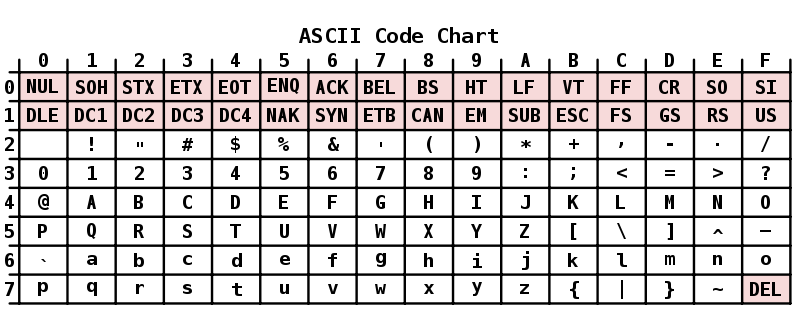
\includegraphics[width=120mm]{./01_basic_types_and_control_flow/800px-ASCII_Code_Chart.png}

Let's take a closer look at some features of the ASCII character set. First,
notice that uppercase and lowercase characters are represented distinctly.
This is why case sensitivity is important on computers. Second, 0 through 31
look really funky. That's because these are called control characters, not
printing characters. Most of these control characters are no longer used in
today's computers (they were used to literally control printers and other
devices in the 70s and 80s), but there are some that warrant special
attention. The first is NULL, 0. NULL is used in C to represent the end of an
array (see Chapter 2). 10, `$\backslash$n' or Newline, is used to make the
computer put a line break in a program's output; otherwise, everything would
show up on one long horizontal line. Second is 15, `$\backslash$r' or Carriage
Return. This goes back to when computer printers were fancy typewriters, which
required a special symbol to move the carriage back to the starting position.
While I can't think of any printers today that need this fuctionality, it is
not uncommon to see `$\backslash$r$\backslash$n' as a legacy pair of
characters in many programs. The last control character that is interesting to
us is 9, `$\backslash$t', horizontal tab. The horizontal tab tells the
computer that we want a lot of whitespace (usually 4 or 8 spaces worth).

\subsection{Strings}

Characters on their own aren't particularly interesting. What is useful is
having long runs of characters to make up words, sentences, paragraphs, and so
on. We achieve this by using what are called strings--- which are literally
just a collection of characters in a row. Usually strings are surrounded by
double quotes in a program. See the workbook for a variety of examples on how
strings look and work in a program.

While characters really are treated as just numbers, strings have a variety of
common operations that don't make sense with numbers. Among these are
operations to determine the length of a string (how many characters it has),
to combine strings together, and to pull strings apart. These are also covered
in detail in the workbook.

\section{Control Flow}

\subsection{Blocks}

\subsubsection{Expression}

\subsubsection{Statement}

\subsection{Branching}

\subsubsection{If-Then-Else}

%\subsubsection{Cases}

\subsection{Looping}

\subsubsection{For Range}

\subsubsection{While}

\section{Comments}

There is one last piece of a program we need to mention. Comments are text in
our programs that are not used by the computer, but are purely for
